% Exercise ID: MAT_A12OTIMI_ESTU_MRE_003
% Module: Módulo A12 - Otimização | Concept: Estudo da Monotonia
% Type: monotonia_real | Difficulty: 2/5
% Tags: monotonia, gráfico, contexto_real, temperatura, quadratica, linear
% Author: Professor | Date: 2025-11-26

\exercicio{
Durante uma experiência, a temperatura de um líquido foi registada ao longo de 2 horas. Inicialmente, o líquido aquece rapidamente, depois arrefece de forma linear. O gráfico mostra a evolução da temperatura ao longo do tempo.

\begin{center}
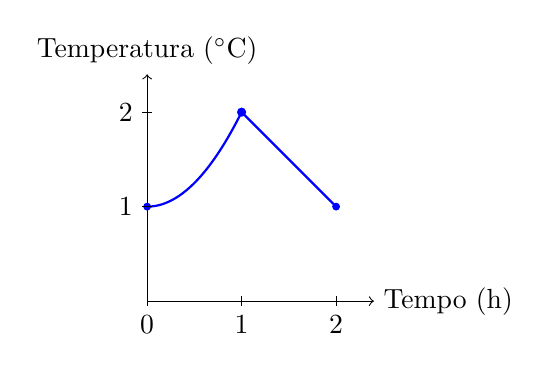
\begin{tikzpicture}[scale=1.2]
  \draw[->] (0,0) -- (2.4,0) node[right] {Tempo (h)};
  \draw[->] (0,0) -- (0,2.4) node[above] {Temperatura ($^\circ$C)};
  % ramos
  \draw[thick, blue, domain=0:1, samples=50] plot (\x, {\x*\x+1});
  \draw[thick, blue] (1,2) -- (2,1);
  % pontos
  \filldraw[blue] (0,1) circle (1pt);
  \filldraw[blue] (1,2) circle (1.2pt);
  \filldraw[blue] (2,1) circle (1pt);
  % marcas x
  \foreach \x in {0,1,2} \draw (\x,0.05) -- (\x,-0.05) node[below] {\x};
  % marcas y
  \foreach \y in {1,2} \draw (0.05,\y) -- (-0.05,\y) node[left] {\y};
\end{tikzpicture}
\end{center}
}

\subexercicio{Durante que intervalo de tempo a temperatura esteve a aumentar?}

\subexercicio{Durante que intervalo de tempo a temperatura esteve a diminuir?}

\subexercicio{Qual foi a temperatura máxima atingida e em que hora isso aconteceu?}

\subexercicio{Interpreta o significado dos diferentes ramos do gráfico no contexto da experiência.}
